% --------------------------------------------------------------
% This is all preamble stuff that you don't have to worry about.
% Head down to where it says "Start here"
% --------------------------------------------------------------
 
\documentclass[12pt]{article}
 
\usepackage[margin=1in]{geometry} 
\usepackage{amsmath,amsthm,amssymb}
\usepackage{mathtools}
\usepackage{graphicx}
\graphicspath{ {img/} }

\newcommand{\N}{\mathbb{N}}
\newcommand{\Z}{\mathbb{Z}}
 
\newenvironment{theorem}[2][Theorem]{\begin{trivlist}
\item[\hskip \labelsep {\bfseries #1}\hskip \labelsep {\bfseries #2.}]}{\end{trivlist}}
\newenvironment{lemma}[2][Lemma]{\begin{trivlist}
\item[\hskip \labelsep {\bfseries #1}\hskip \labelsep {\bfseries #2.}]}{\end{trivlist}}
\newenvironment{exercise}[2][Exercise]{\begin{trivlist}
\item[\hskip \labelsep {\bfseries #1}\hskip \labelsep {\bfseries #2.}]}{\end{trivlist}}
\newenvironment{problem}[2][Problem]{\begin{trivlist}
\item[\hskip \labelsep {\bfseries #1}\hskip \labelsep {\bfseries #2.}]}{\end{trivlist}}
\newenvironment{question}[2][Question]{\begin{trivlist}
\item[\hskip \labelsep {\bfseries #1}\hskip \labelsep {\bfseries #2.}]}{\end{trivlist}}
\newenvironment{corollary}[2][Corollary]{\begin{trivlist}
\item[\hskip \labelsep {\bfseries #1}\hskip \labelsep {\bfseries #2.}]}{\end{trivlist}}

% better formatting of large fractions
\newcommand\ddfrac[2]{\frac{\displaystyle #1}{\displaystyle #2}}
 
\begin{document}
 
% --------------------------------------------------------------
%                         Start here
% --------------------------------------------------------------
 
\title{EE 5630: Optimal Control - Assignment 1}%replace X with the appropriate number
\author{Joshua Saunders\\ %replace with your name
} %if necessary, replace with your course title
 
\maketitle

%---------------
% Question 1
%---------------

\begin{question}{1}
\end{question}
\textbf{Example 2.2-1} describes a process in which a performance measure and 
associated weights can be determined for controlling the attitude, $\theta(t)$, 
of a manned spacecraft using gas expulsion system, shown in Figure \ref{fig:spacecraft_acs}.
The objective of the control system is to maintain the attitude of the
spacecraft at $\theta(t) = 0$ and to do with with small accelerations.

\begin{figure}[h]
    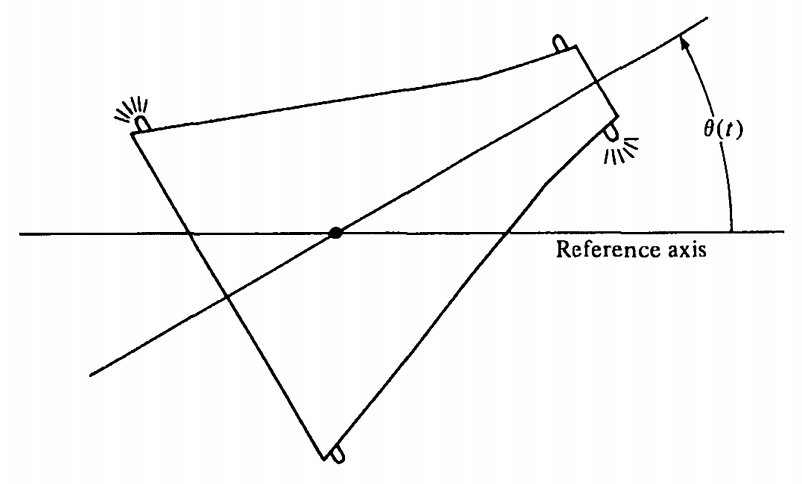
\includegraphics[scale=0.35]{spacecraft_acs}
    \centering
    \caption{Attitude control of a spacecraft \cite{kirkdover}}
    \label{fig:spacecraft_acs}
\end{figure}

The dynamics of the system are given by the differential equation given in 
Equation \ref{eq:spacecraft_acs} and the performance measure is given in
Equation \ref{eq:spacecraft_pf}.

\begin{equation}
    I \ddot{\theta}(t) = \lambda(t) \label{eq:spacecraft_acs}
\end{equation}

and

\begin{equation}
    J = \int_{0}^{\infty} [q_{11} x_1^2(t) + q_{22} x_2^2(t) + R u^2 (t)] \, dt 
    \label{eq:spacecraft_pf}
\end{equation}

\noindent where $I$ is angular moment of inertia and $\lambda(t)$ is the 
torque produced by the gas jets.
\noindent where $u(t) = \dfrac{1}{I} \lambda(t)$. The state space equations are

\begin{align}
    \dot{x_1}(t) &= x_2 (t) \label{eq:sc_ssr_s1} \\
    \dot{x_2}(t) &= u (t) \label{eq:sc_ssr_x2}
\end{align}

%---------------
% Question 2
%---------------

\newpage
\begin{problem}{2-1} %You can use theorem, exercise, problem, or question here.  Modify x.yz to be whatever number you are proving
%Delete this text and write theorem statement here.
\end{problem}
 
The states for the mixing process from \textbf{Problem 1-6} are given by

\begin{equation}
\dot{v}_1 (t) 
\begin{dcases}
    m(t) - \ddfrac{v_1(t) \, k}{\alpha _1 }[h_1(t) \, - \, h_2(t)],  \, & \text{if } h_1(t) \leq h_2(t) \\
    m(t) + \ddfrac{v_2(t) \, k}{\alpha _2 }[h_2(t) \, - \, h_1(t)],  \, & \text{if } h_2(t) > h_1(t) 
\end{dcases}
\end{equation}

and

\begin{equation}
\dot{v}_2 (t) 
\begin{dcases}
    - \ddfrac{v_1(t) \, k}{\alpha _1 }[h_1(t) \, - \, h_2(t)],  \, & \text{if } h_1(t) \leq h_2(t) \\ 
      \ddfrac{v_2(t) \, k}{\alpha _2 }[h_2(t) \, - \, h_1(t)],  \, & \text{if } h_2(t) > h_1(t). 
\end{dcases}
\end{equation}

\noindent \textbf{a)} \newline

The type of problem defined here is a \textit{tracking problem}. Here, the $v_2 (t)$ state is to be kept
as close to $M$ ft\textsuperscript{3} as possible. Therefore, a performace measure that can be used is

\begin{equation}
    J = \int_{t_0}^{t_f} [v_2 (t) \, - \, M]^2 dt
\end{equation}

\noindent
where $t_0$ and $t_f$ are the initial and final times, respectively, and $t_f \, - \, t_0 = 1$ day.

$\\$

\noindent \textbf{b)} \newline

A set of physically realistic state and control constraints are

\begin{align}
    0 \, & \leq \, h_1 (t) \, \leq H_1, \\
    0 \, & \leq \, h_2 (t) \, \leq H_2, \\
    0 \, & \leq \, w_1 (t) \, \leq W_1, \\
    0 \, & \leq \, w_2 (t) \, \leq W_2, \\
    0 \, & \leq \, m (t) \, \leq M
\end{align}

where 

\begin{itemize}
    \item $H_1$ and $H_2$ are the maximum heights of tanks 1 and 2, respectively
    \item $W_1$ and $W_2$ are the maximum rates of water entering tanks 1 and 2, respectively
\end{itemize}

%---------------
% Question 3
%---------------

\newpage
\begin{problem}{2-2}
\end{problem}
 
This type of problem is classified as a \textit{terminal control problem} in which a parameter
is being \textit{maximized} in which the final total volume of dye in tank 2 is to be as close
to $N$ ft\textsuperscript{3} as possible.

$$\\$$
\noindent \textbf{a)} \newline

A performance measure that can be used is

\begin{equation}
    J = - v_2 (t_f) \,.
\end{equation}

\noindent A minus sign is being used because the quantity $v_2(t_f)$ is being \textit{maximized}.

$$\\$$
\noindent \textbf{b)} \newline

A set of physically realizable state and control constraints are

\begin{align}
    0 \, \leq \, h_1 (t) \, & \leq H_1, \\
    0 \, \leq \, h_2 (t) \, & \leq H_2, \\
    0 \, \leq \, w_1 (t) \, & \leq W_1, \\
    0 \, \leq \, w_2 (t) \, & \leq W_2, \\
    \int_{t_0}^{t_f} m (t) \, dt \, & \leq N 
\end{align}

\noindent where 

\begin{itemize}
    \item $H_1$ and $H_2$ are the maximum heights of tanks 1 and 2, respectively
    \item $W_1$ and $W_2$ are the maximum rates of water entering tanks 1 and 2, respectively
    \item where $t_0$ and $t_f$ are the initial and final times, respectively, and $t_f \, - \, t_0 = 1$ day
\end{itemize}

%---------------
% Question 4
%---------------

\newpage
\begin{problem}{2-3}

\end{problem}

%---------------
% References
%--------------
\newpage
\bibliography{bib}
\bibliographystyle{ieeetr}
% --------------------------------------------------------------
%     You don't have to mess with anything below this line.
% --------------------------------------------------------------
 
\end{document}
